\section{Durchführung}
\label{sec:Durchführung}
Hier soll die Filmstreifenmethode verwendent werden,
um zwei Strukturbestimmungen
sowohl von einem Metall als auch von
einem Salz durchzuführen.
% \subsection{Aufbau}
% \label{subsec:Aufbau}
Die Apparatur für die Filmstreifenmethode besteht aus einem hohlen flachen Metallzylinder.
mit eine Öffnung besitzt in der ein Kollimatorrohr eingebaut ist.
Somit fallen gebündelten Röntgenstrahlen auf die Probe die sich in
der Mitte des Metallzylinders befindet.
Die zu bestimmende Probe wird dabei auf ein zylindischen Glasstab
als kristallines Pulver aufgetragen und in der Mitte an einer drehbaren
Achse befestigt. Unter Rotlicht wird ein Filmstreifen an die Innenseite
des Zylinders befestigt und der Zylinder verschlossen.
Mit Hilfe einer Röntgenröhre wird Röntgenstrahlung erzeugt
wobei durch ein $\beta$-Filter die zusätzliche
$\mathrm{K}_\beta$-Strahlung absorbiert wird.
Die verbleibende nicht trennbare  $\mathrm{K}_{\alpha_1}-$
und $\mathrm{K}_{\alpha_2}$-Strahlung fällt durch das Kollimatorrohr
auf die sich im Zyinder befindende Probe. Die Röntgenstrahlen werden an
der Probe an bestimmte Ebenenescharen gebeugt. Für bestimmte Winkel $\theta$ treten
somit Reflexe auf, die als Kegelmantel mit einem Öffnungswinkel von $2\theta$
vorliegen. In der Abbildung \ref{fig:aufbau} ist ein Schematischer Aufbau des Versuches dargestellt.
\begin{figure}
  \centering
  \includegraphics{Aubau.pdf}
  \caption{Schematischer Aufbau des Versuches  }
  \label{fig:aufbau}
 \end{figure}
Nach der Einstrahlungszeit wird der Filmstreifen unter Rotlicht
aus dem Zylinder entnommen und entwickelt.
Dabei wird wie folgt vorgegangen.
Zu Beginn wird der Film im Entwickler $\SI{15}{\min}$ geschwenkt,
danach unter Wasser $\SI{1}{\min}$ abspült.
Unterbrecher
Wieder $\SI{1}{\min}$ unter Wasser
5min Fixierer
5-10min in wasser
30 min Trockenschrank


\subsection{systematische Fehler}
Bei der Messung des Winkels $\theta$
treten durch den Aufbau bedingte zwei systematische Fehler auf.
Zum einem wird der $\theta$-Winkel grundsätzlich zu groß gemessem.
Durch überwiegende Absorption von Röntgenstrahlung in der Probe
findet die Beugung an der Oberfläche des
Probezylinders statt. In Abbildung \ref{fig:error1} wird
der Fehler graphisch dargestellt und nach Bradley und Jay
ergibt sich für die Korrektur
$\Delta \mathrm{a}_\mathrm{A}$
zu Gitterkonstante $\mathrm{a}$
\begin{align}
  \frac{\Delta \mathrm{a}_\mathrm{A}}{\mathrm{a}}=\frac{\rho}{2\mathrm{R}}\left(1-\frac{\mathrm{R}}{\mathrm{F}}\right)\frac{\cos^2\theta}{\theta}.
\end{align}
Dabei entspricht $\rho$ dem Radius der Probe, $R$ dem Kameraradius
und F dem Abstand Fokus-Probe.

 \begin{figure}
   \centering
   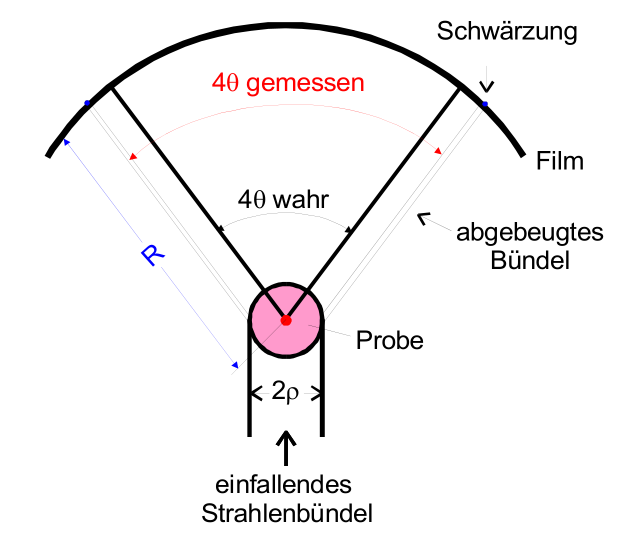
\includegraphics{Syst_error_1.pdf}
   \caption{  }
   \label{fig:error1}
  \end{figure}

Zum andern fallen die Zylinderachsen von Probe und Filmstreifen
nur bedingt ineinander dargestellt in Abbildung \ref{fig:error2}.

\begin{figure}
  \centering
  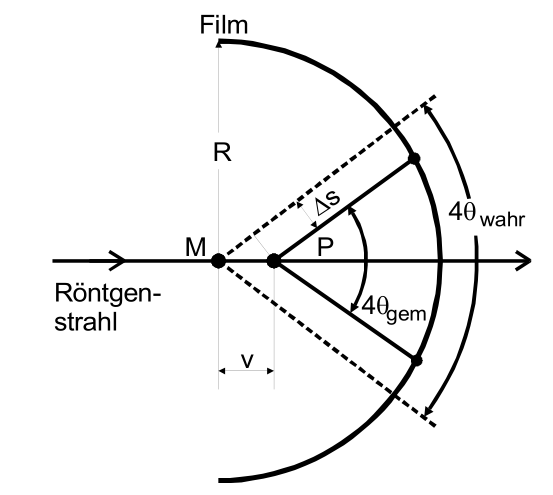
\includegraphics{Syst_error_2.pdf}
  \caption{  }
  \label{fig:error2}
\end{figure}
Der Abstand $v$ der zwei Zylinderachsen in der Röntgenstrahlebene
verändert somit den gemessenen Winkel $\theta$.
Für die Korrektur $\Delta a_\mathrm{V}$ an der Gitterkonstante $\mathrm{a}$
aus diesem systematischen Fehler ergibt sich somit
\begin{align}
  \frac{\Delta a_\mathrm{V}}{\mathrm{a}}=\frac{\mathrm{v}}{\mathrm{R}} \cos^2 \theta.
\end{align}
